\newSec[Quads]{\Quad\ als System}{1}





\newSec{Orientierungsmerkmale}{2}




\begin{figure}[ht!]
\vspace{0.25cm}
\begin{center}
\fbox{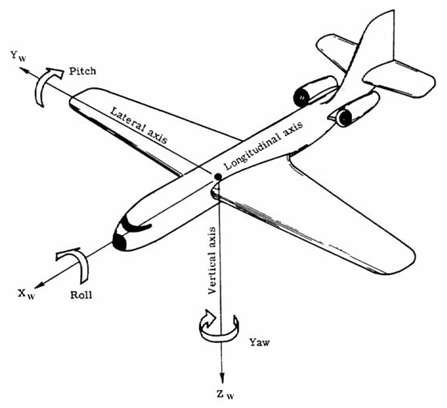
\includegraphics[width=12cm]{Pictures/Orientations.png}}
\caption{Orientierungsmerkmale eines Flugobjekts \cite{parotSDK}}
\label{fig:Orient}
\end{center}

\vspace{0.25cm}
\refImgShort{fig:Orient} zeigt die Orientierung eines beliebigen Flugobjektes am beispiel eines Flugzeugs. Die Bezeichner beziehen sich auf ein kartesisches Korrdinatensystem und beschrieben jeweils die Rotation um eine Raumachse.
\end{figure}






\newSec{Geometrien}{2}
Bei \Quad[n] handelt es sich im allgemeinen um Fluggeräte mit vier Rotoren, welche horizontal angebracht sind. Der Auftrieb wird somit unmittelbar durch die Rotoren induziert.

Die Rotoren von \Quad[n] können in zwei verschiedenen Anordnungen angebracht werden. In diesem Kapitel sollen diese Anordnung näher beschrieben werden.




\begin{figure}[ht!]
\vspace{0.25cm}
\begin{center}
\fbox{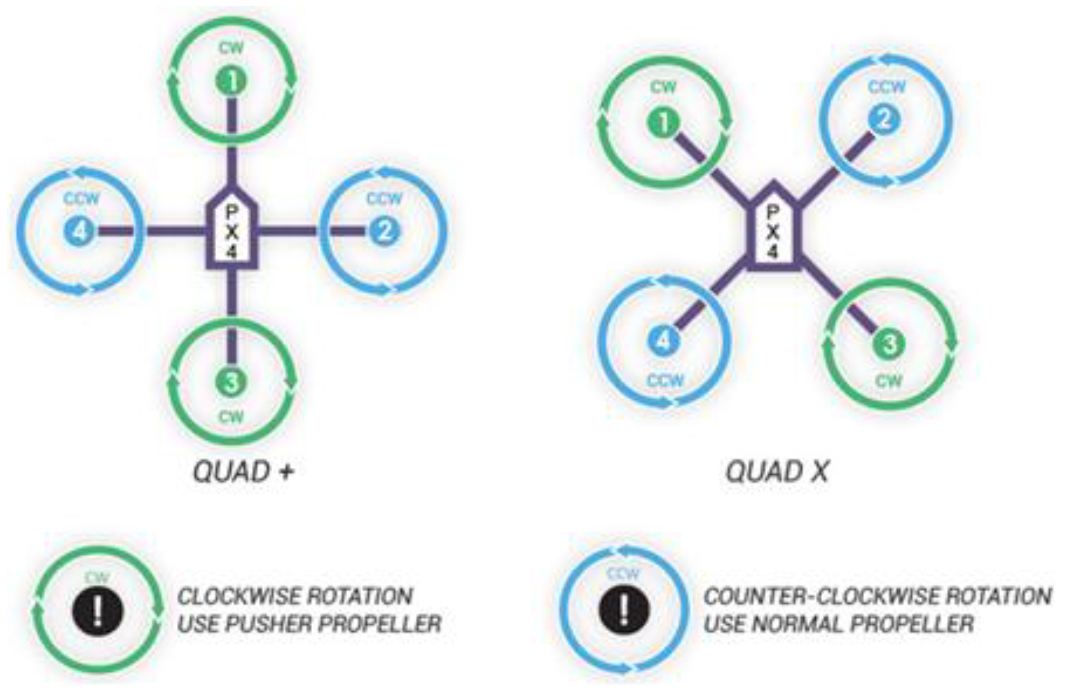
\includegraphics[width=12cm]{Pictures/Geometries.png}}
\caption{Geometrien von \Quad[n] \cite{Paper1}}
\label{fig:Geom}
\end{center}

\vspace{0.25cm}
\refImgShort{fig:Geom} zeigt \missing.
\end{figure}


Das Drehmoment der Rotoren des \Quad[s] muss sich aufheben können, um eine unkontrollierbare Rotation um die z-Achse vermeiden zu können. Um die Agilität des \Quad[s] beibehalten zu können, sind die Drehrichtungen der Rotoren zu alternieren.\comp{Paper1}


\newSec[Plus]{\textbf{+}-Anordnung}{3}

In der \textbf{+}-Anordnung befinden sich die Rotoren auf den Lokalen Achsen des \Quad[s]. Die Nummerierung der Rotoren erfolgt gemäß \refImg{fig:Geom} (links) im Uhrzeigersinn beginnend mit dem Rotor auf der positiven x-Achse.


\missing[für roll und pitch wird die Drehzahl die Rotoren auf der jeweiligen Achse entgegengesetzt angepasst.]
\missing[für eine Drehung um die z-Achse (yarn) werden die Rotoren der x- und y-Achse entgegengesetzt manipuliert.]



\newSec[X]{\textbf{x}-Anordnung}{3}
\missing\








\newSec{Freiheitsgrade}{2}




6 Freiheitsgrade, tatsächlich 4 individuell regelbar.

\missing[Bild der Kräfte an der Drohne, wenn diese aus der horizontalen Ebene geneigt ist.]



\begin{figure}[ht!]
\vspace{0.25cm}
\begin{center}
\fbox{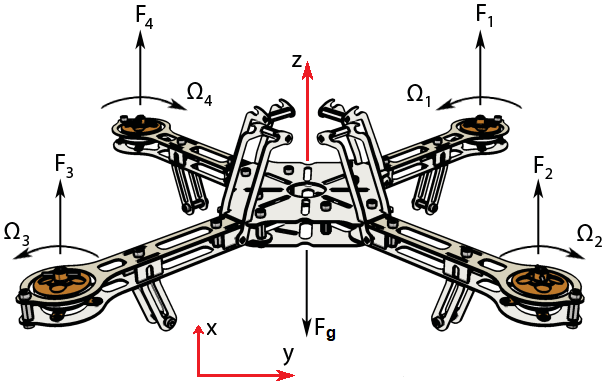
\includegraphics[width=12cm]{Pictures/Forces.png}}
\caption{wirkende Kräfte am \Quad\ in \textbf{x}-Anordnung \comp{Paper2}}
\label{fig:Forces}
\end{center}

\vspace{0.25cm}
\refImgShort{fig:Forces} zeigt die wirkenden Kräfte an einem \Quad\ in \textbf{x}-Anordnung. Die Achsen das Koordinatensystems sind in \textcolor{red}{rot} markiert. Alle mit \textit{F} markeirten Pfeile deuten Kräfte an. Die mit \missing[Omega] markierten gebogenen Pfeile zeigen die Rotationsgeschwindigkeit der einzelnen Rotoren.



 Orientierung eines beliebigen Flugobjektes am beispiel eines Flugzeugs. Die Bezeichner beziehen sich auf ein karthesisches Korrdinatensystem und beschrieben jeweils die Rotation um eine Raumachse.
\end{figure}







\begin{figure}[ht!]
\vspace{0.25cm}
\begin{center}
\fbox{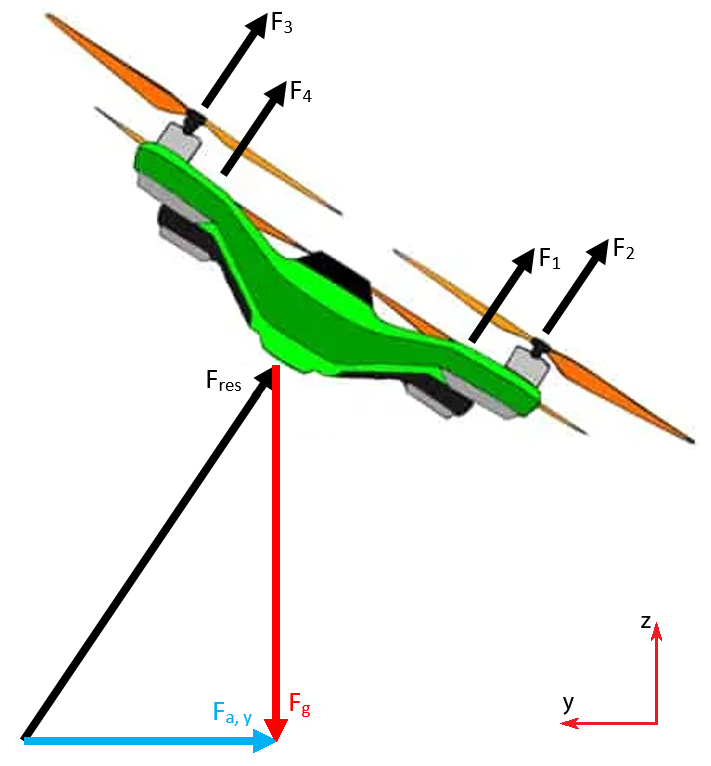
\includegraphics[width=12cm]{Pictures/Forces_Rolled.png}}
\caption{wirkende Kräfte für gerollten \Quad\ \comp{Quad1}}
\label{fig:ForcesRolled}
\end{center}

\vspace{0.25cm}
\refImgShort{fig:ForcesRolled} zeigt die auf einen \Quad\ wirkenden Kräfte, wenn sich dieser in einer gerollten Orientierung befindet. Hier entspricht der Betrag der Kraft entlang der z-Achse der Gewichtskraft.
\end{figure}


Die Kraft $F_{res}$ wird mit der Gewichtskraft $F_g$ überlagert. Die hieraus resultierende Kraft kann in zwei Kräfte aufgeteilt werden, welche parallel zu den kartesischen Achsen angeordnet sind. Hieraus kann berechnet sich die Beschleunigung, welche auf den \Quad\ wirkt.

\missing[muss hier eine Quelle angegeben werden? Wenn ja, evtl. Vorlesung tech Mech aus MB13VT.]




Hieraus ergibt ich, dass eine Neigung zur horizontalen Ebene ine Beschleunigung in der horizontalen Ebene induziert wird. Somit ist jede Position auf der horizontalen Ebene von der Neigung zu dieser Ebene abhängig. Daraus folgt die Reduktion der Freiheitsgrde von sechs auf vier.

\missing[hier vielleicht noch ne Quelle...]









\newSec{Pose}{2}
Eine Pose ist die Positions- und Lagebeschreibung in einem Raum. \missing[quelle]










\newSec{lokale Pose}{3}




\newSec{globale Pose}{3}











